% author cany
\documentclass{beamer}

\usepackage{graphicx}
\usepackage{amsmath}
\usepackage{biblatex}
\usepackage{hyperref}
\usepackage{listings}
\usepackage{caption}
\usepackage{ amssymb }
\usepackage[utf8]{inputenc}
\usepackage{refcount}
\usepackage{tikz}
\usepackage{amssymb}
\usepackage{color, colortbl}
\usepackage{booktabs,array}  
\usepackage{caption}
\usepackage{bm}
\usepackage{verbatim}
\usepackage{listings}
\usepackage{svg}

\usefonttheme{professionalfonts}
\captionsetup[lstlisting]{singlelinecheck=false, margin=0pt, font={sf,sl,footnotesize}}


\lstset{%
	language=Python,
	basicstyle=\ttfamily\footnotesize,
	frame=lines,
	keywordstyle=\color{blue}\textbf,
	commentstyle=\color[rgb]{0.0,0.4,0.0}\scriptsize,
	extendedchars=true,         
	breaklines=true,           
	xleftmargin=0.2cm
}

\mode<presentation>
{
	\usetheme{Madrid}
	\setbeamercovered{transparent}
	\setbeamertemplate{caption}[numbered]
}
\beamertemplatenavigationsymbolsempty

\newcommand\pro{\item[$+$]}
\newcommand\con{\item[$-$]}

\title[B-IT Pattern Recognition] {B-IT Pattern Recognition}
\subtitle { Project-I Report } 
\author[]{Students: \textit{Mohammadali Ghasemi, Chu-I Chao, Neng Qian,\\ Vanik Karslian, Can Yuce}
 }
\institute[B-IT] 
{
	Bonn-Aachen International Center for \\ Information Technology(B-IT)\\
}
\date{\today}
\setbeamertemplate{enumerate items}[square]
  \setbeamertemplate{itemize items}[square]
  
\begin{document}
	
	\begin{frame}
		\titlepage
	\end{frame}
	
	
	\begin{frame}{Outline}
		\tableofcontents
	\end{frame}
	
	
\section{Generalities}

\begin{frame}{Generalities}
	\structure{Programming Language, Libraries:}
	\begin{itemize}
    	\item Implementation of the solution is in \structure{Python}.
    	\item Using \structure{NumPy}, \structure{SciPy}, \structure{Matplotlib} modules.
    	\item Anaconda data science platform\footnote{https://www.anaconda.com/} (not obligatory).
	\end{itemize}
	\begin{figure}
		\centering
		
\includegraphics[width=0.4\textwidth]{images/python-snake.jpg}
		\label{label1}
	\end{figure}
\end{frame}

\section{Task 1.1: Plotting 2D data}
\begin{frame}[fragile]{Task 1.1: Plotting 2D data}
	\begin{itemize}
		\item \textbf{Task:} Plotting the data without the outliers,
		\item \textbf{Why?}
		\begin{itemize}
		    \item To deal with missing data,
		    \item To deal with outliers.
	    \end{itemize}
		\item \textbf{How?} 
		 \newline
		 \newline
		  A Python Code Sample:
\begin{lstlisting}[linewidth=8.4cm]
# Task 1.1 
outlierInd = np.where( X[:,0] != -1 ) 
X, y = X[outlierInd], y[outlierInd]
\end{lstlisting}
\end{itemize}

\end{frame}


\begin{frame}{Task 1.1: Plotting 2D data}

\begin{figure}
	\centering
	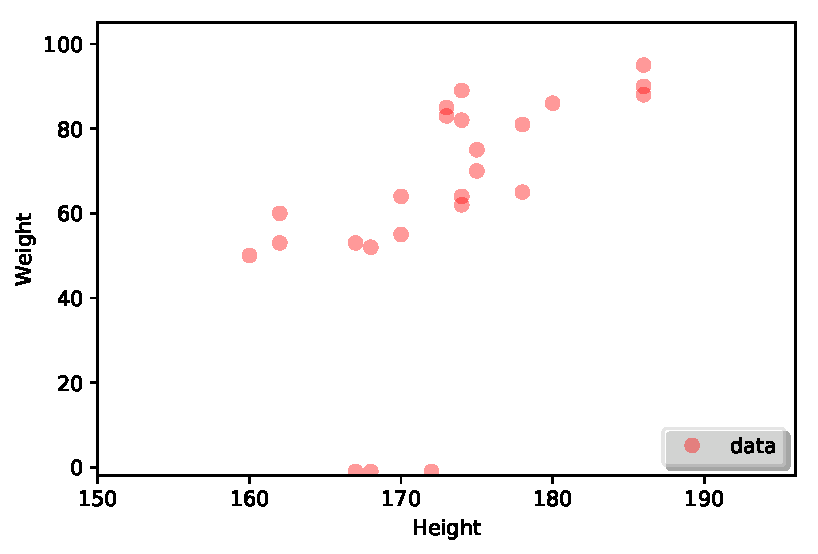
\includegraphics[width=.4\textwidth]{images/plotHW_outl.pdf}\quad
	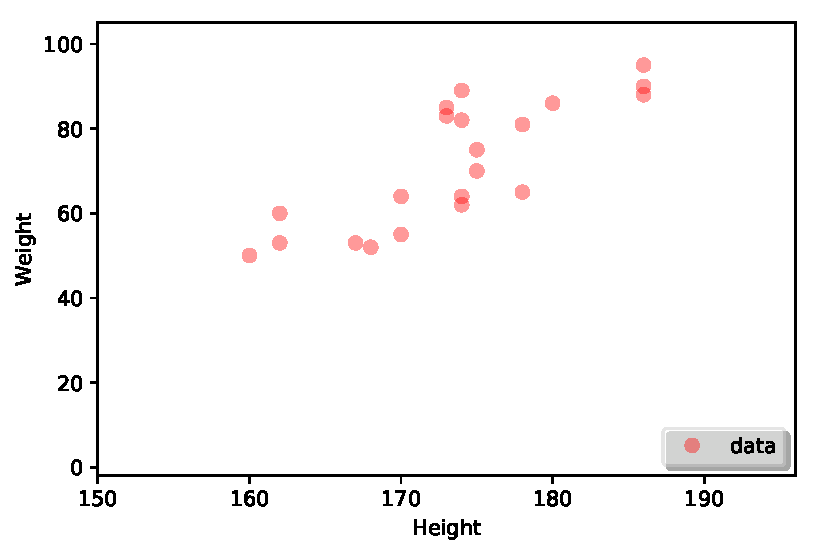
\includegraphics[width=.4\textwidth]{images/plotHW.pdf}
	
	\medskip
	
	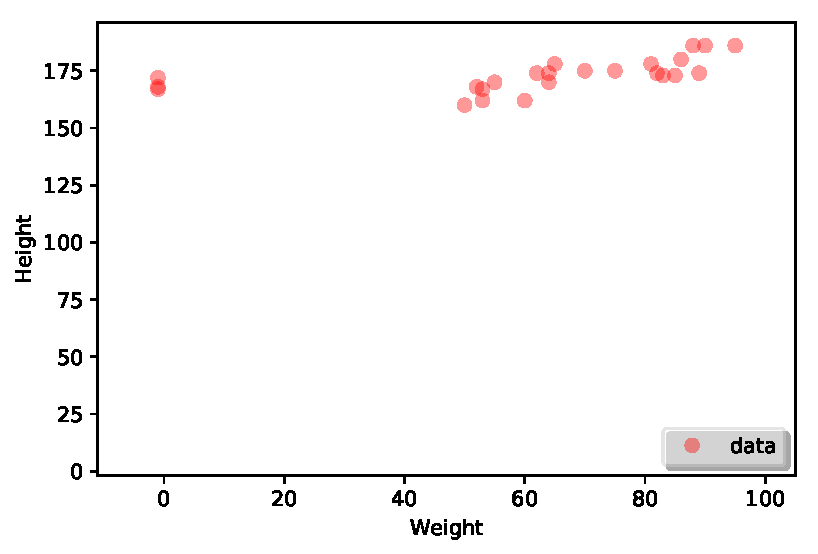
\includegraphics[width=.4\textwidth]{images/plotWH_outl.pdf}\quad
	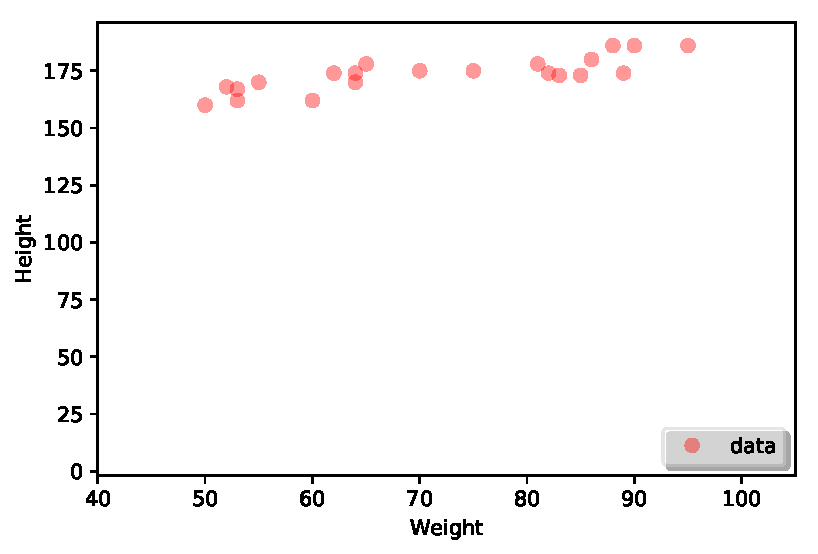
\includegraphics[width=.4\textwidth]{images/plotWH.pdf}
	
	\caption{Removing outliers.}
\end{figure}

\end{frame}

\begin{frame}[fragile]{Task 1.1: Plotting 2D data}

\begin{columns}
\begin{column}{0.35\textwidth}
	\hspace{1cm}
\begin{lstlisting}[linewidth=5.0cm]
# Task 1.1
axs.set_aspect('equal')
\end{lstlisting}
\begin{itemize}
	\item same scaling from data to plot units for $x$ and $y$,
\end{itemize}
\end{column}


\begin{column}{0.65\textwidth}  
\begin{figure}
	\centering
	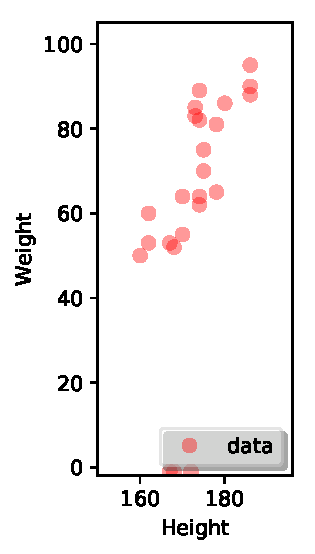
\includegraphics[width=.3\textwidth]{images/plotHW_equal_aspect_ratio_outl.pdf}\quad
	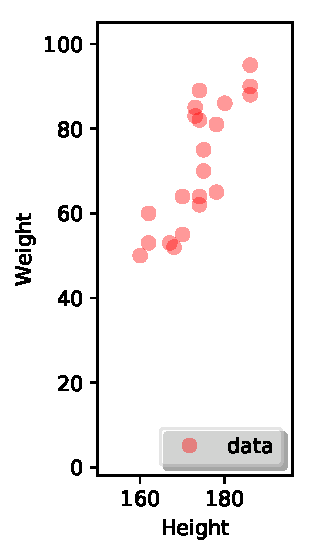
\includegraphics[width=.3\textwidth]{images/plotHW_equal_aspect_ratio.pdf}
	\caption{Plots with equal aspect ratio.}
\end{figure}
\end{column}
\end{columns}

\end{frame}

\section{Task 1.2: Fitting a Normal Distribution on 1D Data}

\begin{frame}{Task 1.2: Fitting a Normal Distribution on 1D Data}
\begin{itemize}
	\item \textbf{Task:} 
	\begin{itemize}
		\item Calculate the mean and standard deviation of body sizes,
		\item Plot the data and normal distribution.
	\end{itemize}
	\item \textbf{Why?}
	\begin{itemize}
		\item To be sure that body sizes are distributed accordingly to normal distribution.
	\end{itemize}
	\item \textbf{How?} 
	\begin{itemize}
		\item Using ML estimation:
	\end{itemize}
		\begin{align*}
	\text{ Normal Distribution: } f(x|\mu,\sigma^2) =& \frac{1}{\sqrt{2\pi\sigma^2}}e^{-\frac{(x-\mu)^2}{2\sigma^2}} \\
	\text{Standard Deviation: } \sigma_{MLE} =& \sqrt{\frac{1}{n}\sum_{i=1}^{n}(x_i-\mu)^2} \\
	\text{Mean: } \mu_{MLE} =& \frac{1}{n}\sum_{i=1}{n}{s_i}
\end{align*}
\end{itemize}
\end{frame}


\begin{frame}{Task 1.2: Fitting a Normal Distribution on 1D Data}
\begin{columns}
\begin{column}{0.5\textwidth}  
\begin{figure}
	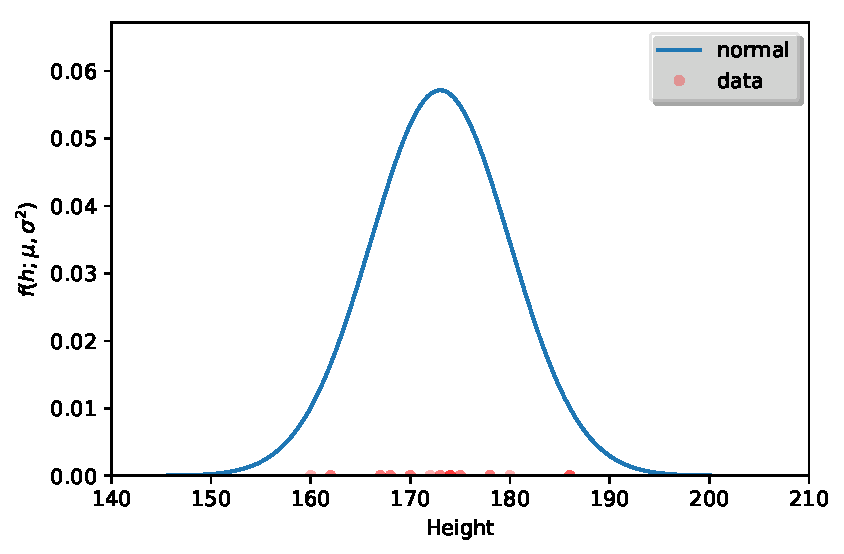
\includegraphics[width=1\textwidth]{images/plotNormal_Height.pdf}	\caption{$\mu_h=173.0, \sigma_h=6.98$}
\end{figure}
\end{column}
\begin{column}{0.5\textwidth}  
	\begin{figure}
		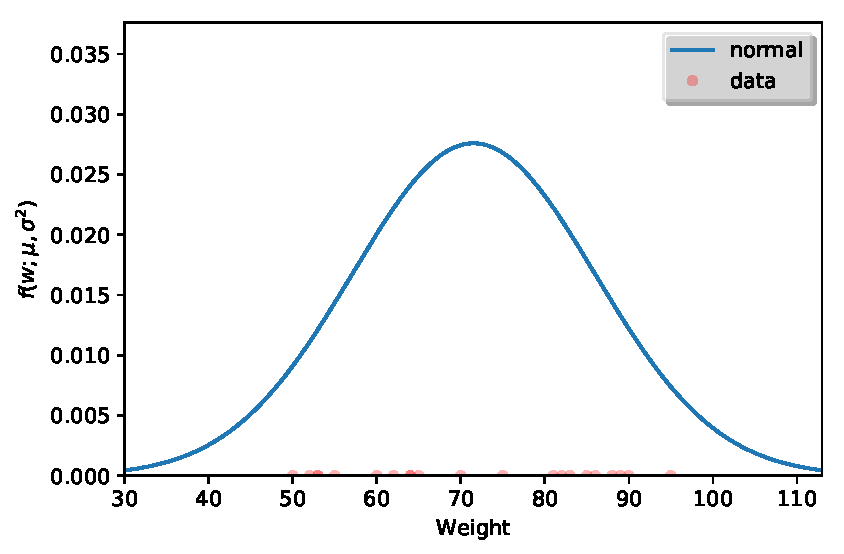
\includegraphics[width=1\textwidth]{images/plotNormal_Weight.pdf} \caption{($\mu_w=71.52, \sigma_w=14.46$)}
	\end{figure}
\end{column}
\end{columns}

\end{frame}

\section{Task 1.3: Fitting Weibull Distribution to 1D Data}
\begin{frame}{Task 1.3: Fitting Weibull Distribution to 1D Data}

\begin{figure}
	\centering
	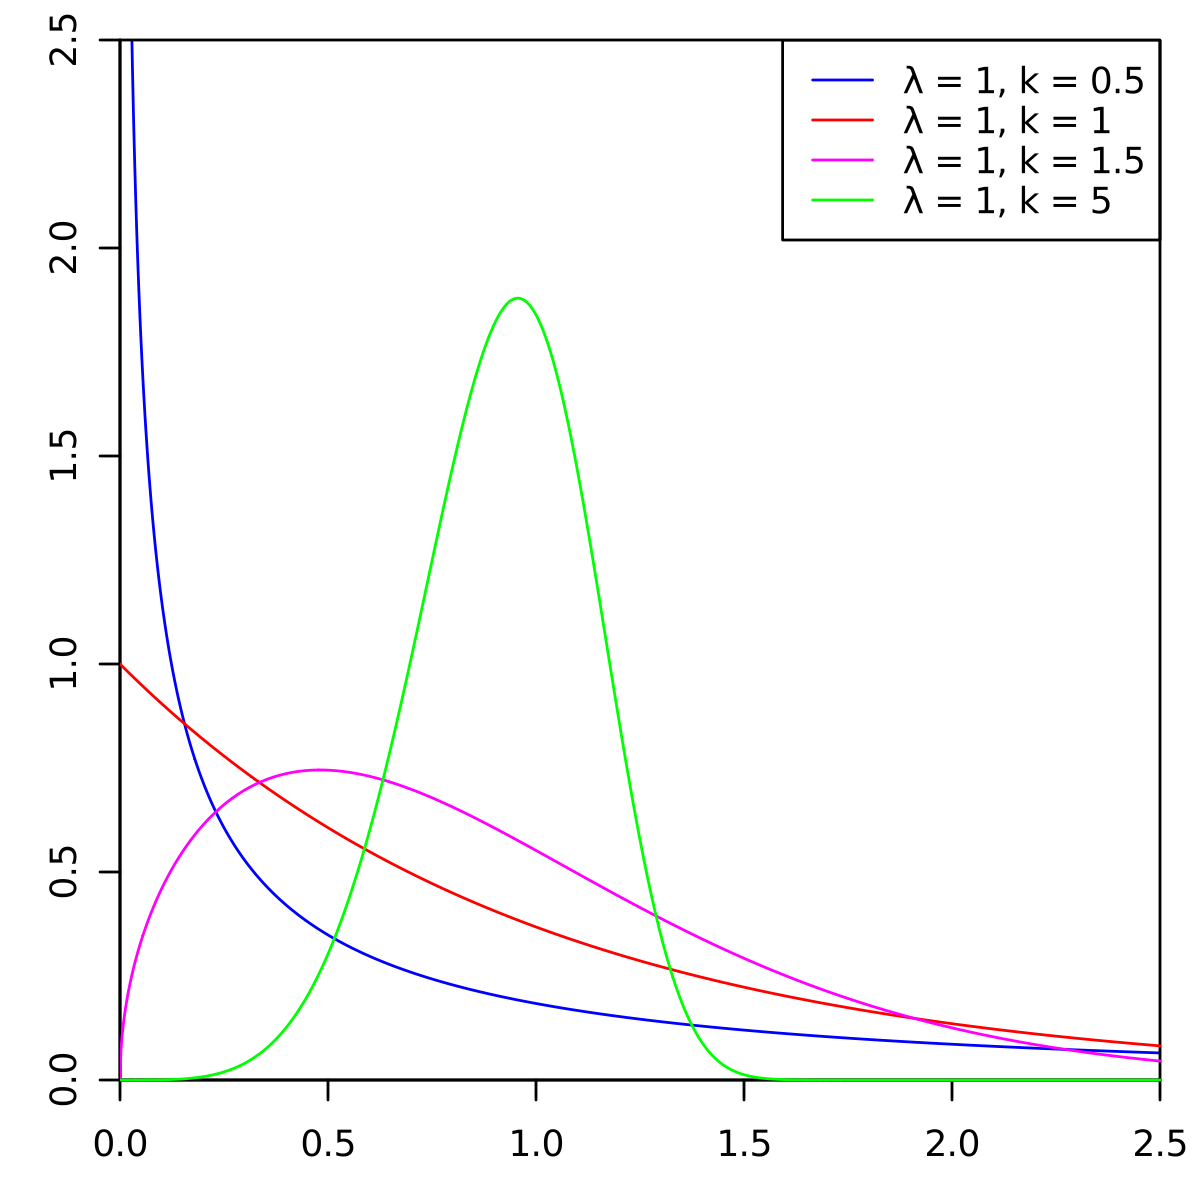
\includegraphics[width=.3\textwidth]{images/weibull.png}
	\caption{Weibull Distribution.}
\end{figure}
\vspace{-0.3cm}
\begin{align*}
&\text{PDF of Weibull distribution: }\\
&f(x|\kappa, \alpha)=\frac{\kappa}{\alpha}\left(\frac{x}{\alpha} \right)^{\kappa-1}e^{-\left( \frac{x}{\alpha}\right)^\kappa}, \text{ if } x\geq 0 \text{ otherwise } 0.  \\
&\text{where } \kappa \text{ is the shape parameter and} \\ 
&\alpha \text{ is the scale parameter.}
\end{align*}
\end{frame}

\begin{frame}{Task 1.3: Fitting Weibull Distribution to 1D Data}
\begin{itemize}
	\item \textbf{Task:} 
	\begin{itemize}
		\item Estimate the parameters of Weibull distribution,
		\item Plot the data and Weibull distribution..
	\end{itemize}
	\item \textbf{Why?}
	\begin{itemize}
		\item To have a good prediction if the Weibull distribution can be closely fitted to the observed data.
	\end{itemize}
	\item \textbf{How?} 
	\begin{itemize}
		\item \structure{Maximum Likelihood Estimation(MLE)}: Estimate $\kappa, \alpha$ which makes the log-likelihood as large as possible.
		\item Use the function \structure{scipy.integrate.odeint}.
	\end{itemize}

\end{itemize}
\end{frame}

\begin{frame}{Task 1.3: Fitting Weibull Distribution to 1D Data}
\begin{itemize}
	\item \textbf{How?} 
	\begin{itemize}
		\item \structure{Maximum Likelihood Estimation(MLE)}: Estimate $\kappa, \alpha$ which makes \\ the log-likelihood as large as possible.
		\begin{align*}
		&\text{PDF of Weibull distribution: }\\
		&f(x|\kappa, \alpha)=\frac{\kappa}{\alpha}\left(\frac{x}{\alpha} \right)^{\kappa-1}e^{-\left( \frac{x}{\alpha}\right)^\kappa}, \\ 
		&\text{Log-likelihood is:} \\
		& L(\alpha,\kappa|D) = N\left( \log\kappa)-\kappa\log(\alpha)\right) + \left( \kappa-1\right) \sum_i{\log d_i} - \sum_i{\left( d_i/\alpha \right)^\kappa }  
		\end{align*}
		\vspace{-0.5cm}
		\item{Use Newton Raphson Method:} \\
		\vspace{-0.5cm}		
		\begin{align*}
		&\begin{bmatrix}
			\kappa^\text{new} \\[6pt]
			\alpha^\text{new}
		\end{bmatrix}
		=
		\begin{bmatrix}
		\kappa\\[6pt]
		\alpha
		\end{bmatrix}
		+
		\begin{bmatrix}
			\frac{\partial^2 L}{\partial \kappa^2} 	\frac{\partial^2 L}{\partial \kappa \partial \alpha}   \\[6pt]
			\frac{\partial^2 L}{\partial \kappa \partial \alpha}  \frac{\partial^2 L}{\partial \alpha^2}
		\end{bmatrix} ^{-1}
		\begin{bmatrix}
		-\frac{\partial L}{\partial \kappa}  \\[6pt]
		-\frac{\partial L}{\partial \alpha}
		\end{bmatrix} 
		\end{align*}
	\item{Run for ~20 iterations.} \\	
	\end{itemize}	
\end{itemize}
\end{frame}

\begin{frame}[fragile]{Task 1.3: Fitting Weibull Distribution to 1D Data}
\begin{itemize}
	\item{Plot the data histogram with the scaled version of the fitted distribution.}
\end{itemize}

\begin{lstlisting}[linewidth=12cm]
def model(y, t):
	K, a = y[0], y[1]
	d_K = N / K - N * math.log(a) + sum_log_di - np.sum( ((hist / a) ** K) *  np.log(hist / a))
	d_a = (K / a) * (np.sum((hist / a) ** K) - N)
	return [d_K, d_a]

# initial condition and  time points
K, a = 1., 1.
t = np.linspace(0,100,1000)
y = odeint(model,[K,a],t)
\end{lstlisting}

\end{frame}


\begin{frame}{Task 1.3: Fitting Weibull Distribution to 1D Data}
\begin{itemize}
	\item{Plot the data histogram with the scaled version of the fitted distribution.}
\end{itemize}

\begin{figure}
	\centering
	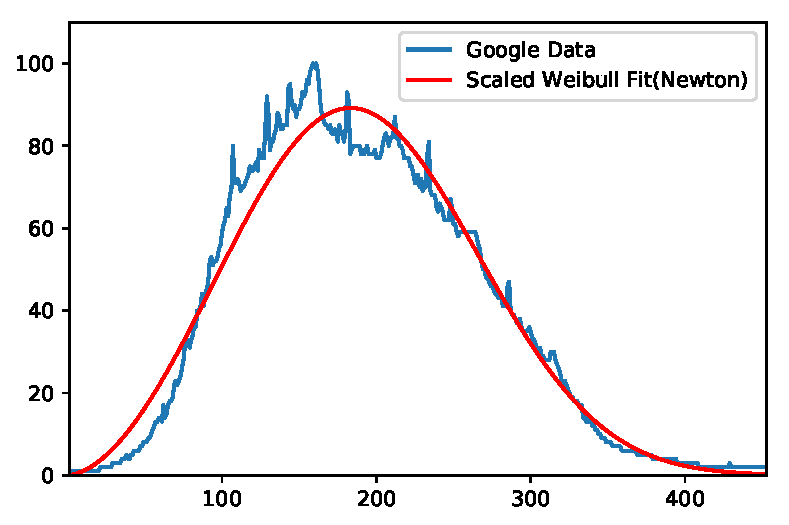
\includegraphics[width=.4\textwidth]{images/fit_newton.pdf}\quad
	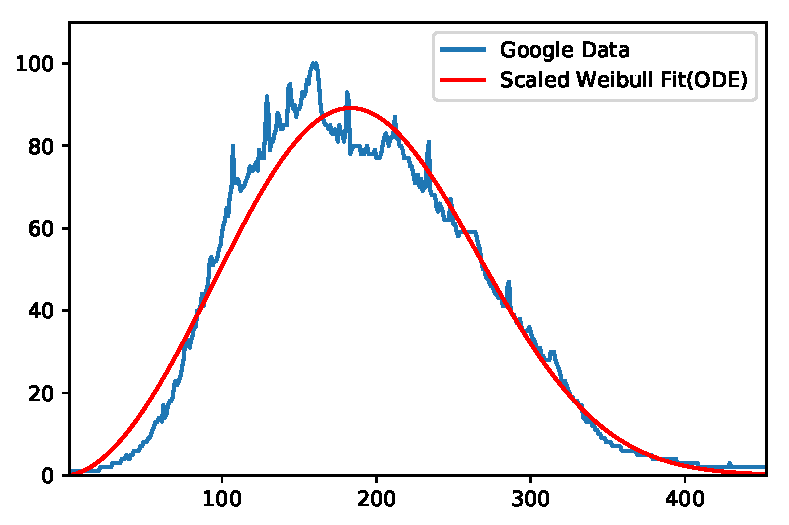
\includegraphics[width=.4\textwidth]{images/fit_ode.pdf}
	\captionsetup{justification=centering}
	\caption{Data fitting with Newton Raphson Method(left) and \\ \structure{scipy.integrate.odeint}(right).}
\end{figure}
\end{frame}

\section{Task 1.4: Drawing Unit Circles}

\section{Task 1.5: Estimating the Dimension of Fractal Objects in an Image}


\end{document}
  
  